\let\negmedspace\undefined
\let\negthickspace\undefined
\documentclass[journal]{IEEEtran}
\usepackage[a5paper, margin=10mm, onecolumn]{geometry}
%\usepackage{lmodern} % Ensure lmodern is loaded for pdflatex
\usepackage{tfrupee} % Include tfrupee package

\setlength{\headheight}{1cm} % Set the height of the header box
\setlength{\headsep}{0mm}     % Set the distance between the header box and the top of the text

\usepackage{gvv-book}
\usepackage{gvv}
\usepackage{cite}
\usepackage{amsmath,amssymb,amsfonts,amsthm}
\usepackage{algorithmic}
\usepackage{graphicx}
\usepackage{float}

\usepackage{textcomp}
\usepackage{xcolor}
\usepackage{txfonts}
\usepackage{listings}
\usepackage{enumitem}
\usepackage{mathtools}
\usepackage{gensymb}
\usepackage{comment}
\usepackage[breaklinks=true]{hyperref}
\usepackage{tkz-euclide} 
\usepackage{listings}
% \usepackage{gvv}                                        
\def\inputGnumericTable{}                                 
\usepackage[latin1]{inputenc}                                
\usepackage{color}                                            
\usepackage{array}                                            
\usepackage{longtable}                                       
\usepackage{calc}                                             
\usepackage{multirow}                                         
\usepackage{hhline}                                           
\usepackage{ifthen}                                           
\usepackage{lscape}
\usepackage{circuitikz}


\renewcommand{\thefigure}{\theenumi}
\renewcommand{\thetable}{\theenumi}
\setlength{\intextsep}{10pt} % Space between text and floats


\numberwithin{equation}{enumi}
\numberwithin{figure}{enumi}
\renewcommand{\thetable}{\theenumi}


% Marks the beginning of the document
\begin{document}
\bibliographystyle{IEEEtran}
\vspace{3cm}

\title{GATE 2024 ES}
\author{EE25BTECH11006 - ADUDOTLA SRIVIDYA}
\maketitle
\noindent
\textbf{Q.1 -- Q.5 Carry ONE mark each}

\vspace{0.5cm}

\begin{enumerate}[start=1, label={Q\arabic*.}]

\item If `$\rightarrow$` denotes increasing order of intensity, then the meaning of the words
$ \text{sick} \rightarrow \text{infirm} \rightarrow \text{moribund}
\quad \text{is analogous to} \quad
\text{silly} \rightarrow \underline{\hspace{1.5cm}} \rightarrow \text{daft} $
Which one of the given options is appropriate to fill the blank?
\begin{enumerate} 
\begin{multicols}{4}
  \item frown
  \item fawn
  \item vein
  \item vain
  \end{multicols}
  \end{enumerate}
\item The 15 parts of the given figure are to be painted such that no two adjacent parts with shared boundaries (excluding corners) have the same color. The minimum number of colors required is
\begin{figure}[H]
    \centering
    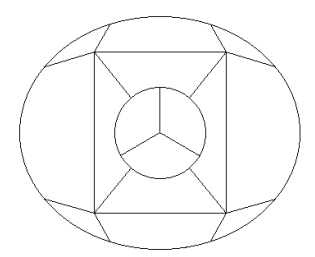
\includegraphics[width=0.3\linewidth]{figs/fig1.png}
    \caption{First figure}
    \label{fig:first}
\end{figure}
\begin{enumerate} 
\begin{multicols}{4}
  \item $4$
  \item $3$
  \item $5$
  \item $6$
  \end{multicols}
  \end{enumerate}
  
\item How many $4$-digit positive integers divisible by $3$ can be formed using only the digits \cbrak{1, 3, 4, 6, 7}, such that no digit appears more than once in a number?
\begin{enumerate} 
\begin{multicols}{4}
  \item $24$
  \item $48$
  \item $72$
  \item $12$
  \end{multicols}
  \end{enumerate}
\item The sum of the following infinite series is 
 \[
 2 + \frac{1}{2} + \frac{1}{3} + \frac{1}{4} + \frac{1}{8} + \frac{1}{9} + \frac{1}{16} + \frac{1}{27} + \cdots                              \]
 \begin{enumerate} 
\begin{multicols}{4}
  \item $11/3$
  \item $7/2$
  \item $13/4$
  \item $9/2$
  \end{multicols}
  \end{enumerate}
  \newpage
\item In an election the share of valid votes received by the four candidates A, B, C, and D is represented by the pie chart shown. The total number of votes cast in the election were $1,15,000$, out of which $5,000$ were invalid
 \begin{figure}[H]
     \centering
     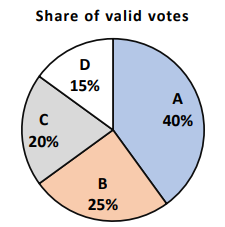
\includegraphics[width=0.5\linewidth]{figs/fig2.png}
     \caption{Sec figure}
     \label{fig:sec}
 \end{figure}
 Based on the data provided, the total number if valid votes received by the candidates B and c is

 \begin{enumerate} 
\begin{multicols}{4}
  \item $45,000$
  \item $49,500$
  \item $51,750$
  \item $54,000$
  \end{multicols}
  \end{enumerate}
 \item Thousands of years ago, some people began dairy farming. This coincided with a number of mutations in a particular gene that resulted in these people developing the ability to digest dairy milk. 
 Based on the given passage, which of the following can be inferred?

\begin{enumerate}
  \item All human beings can digest diary milk.
  \item No human being can digest diary milk.
  \item Digestion of diary milk is essential for human beings.
  \item In human beings, digestion of diary milk resulted from a mutuated gene.
  \end{enumerate}
\item The probability of a boy or a girl being born is 1/2. For a family having only three children, what is the probability of having two girls and one boy?
 \begin{enumerate} 
\begin{multicols}{4}
  \item $3/8$
  \item $1/8$
  \item $1/4$
  \item $1/2$
  \end{multicols}
  \end{enumerate}
  \newpage
\item Person $1$ and Person $2$ invest in three mutual funds A, B, and C. The amounts they invested in each of these mutual funds are given in the table.
\begin{center}
    \begin{tabular}{|c|c|c|c|}
    \hline
    & {Mutual fund A} & {Mutual fund B} & {Mutual fund C} \\
    \hline
    {Person 1} & \rupee10,000 & \rupee20,000 & \rupee20,000 \\
    \hline
    {Person 2} & \rupee20,000 & \rupee15,000 & \rupee15,000 \\
    \hline
    \end{tabular}
\end{center}
At the end of one year, the total amount that Person $1$ gets is \rupee500 more than Person $2$. The annual rate of return for the mutual funds B and C is $15\%$ each. What is the annual rate of return for the mutual fund A?
 \begin{enumerate} 
\begin{multicols}{4}
  \item $7.5\%$
  \item $10\%$
  \item $15\%$
  \item $20\%$
 \end{multicols}
  \end{enumerate}
\item Three different views of a dice are shown in the figure below.
 \begin{center}
\begin{tikzpicture}[scale=1]
\begin{scope}[x={(0.866cm,-0.5cm)}, y={(0cm,1cm)}, z={(0.5cm,0.866cm)}]
  \draw (0,0,0) -- (1,0,0) -- (1,1,0) -- (0,1,0) -- cycle;
  \draw (1,0,0) -- (1,0,1) -- (1,1,1) -- (1,1,0); 
  \draw (0,1,0) -- (0,1,1) -- (1,1,1) -- (1,1,0); 
  \node at (0.5,0.5,0) {1};
  \node at (1,0.5,0.5) {4};
  \node at (0.5,1,0.5) {5};
\end{scope}
\begin{scope}[xshift=3cm, x={(0.866cm,-0.5cm)}, y={(0cm,1cm)}, z={(0.5cm,0.866cm)}]
  \draw (0,0,0) -- (1,0,0) -- (1,1,0) -- (0,1,0) -- cycle;
  \draw (1,0,0) -- (1,0,1) -- (1,1,1) -- (1,1,0); 
  \draw (0,1,0) -- (0,1,1) -- (1,1,1) -- (1,1,0); 
  \node at (0.5,0.5,0) {3};
  \node at (1,0.5,0.5) {6};
  \node at (0.5,1,0.5) {4};
\end{scope}
\begin{scope}[xshift=6cm, x={(0.866cm,-0.5cm)}, y={(0cm,1cm)}, z={(0.5cm,0.866cm)}]
  \draw (0,0,0) -- (1,0,0) -- (1,1,0) -- (0,1,0) -- cycle;
  \draw (1,0,0) -- (1,0,1) -- (1,1,1) -- (1,1,0); 
  \draw (0,1,0) -- (0,1,1) -- (1,1,1) -- (1,1,0); 
  \node at (0.5,0.5,0) {5};
  \node at (1,0.5,0.5) {6};
  \node at (0.5,1,0.5) {2};
\end{scope}
\end{tikzpicture}
\end{center}

The piece of paper that can be folded to make this dice is

 \begin{enumerate} 
\begin{multicols}{2}
  \item 
\begin{center}
\begin{tikzpicture}[scale=1.2]
  \draw (0,0) rectangle ++(1,-1);
  \draw (1,0) rectangle ++(1,-1);
  \draw (1,-1) rectangle ++(1,-1);
  \draw (1,-2) rectangle ++(1,-1);
  \draw (1,-3) rectangle ++(1,-1);
  \draw (2,-3) rectangle ++(1,-1);

  \node at (0.5,-0.5) {5};
  \node at (1.5,-0.5) {1};
  \node at (1.5,-1.5) {4};
  \node at (1.5,-2.5) {6};
  \node at (1.5,-3.5) {2};
  \node at (2.5,-3.5) {3};
\end{tikzpicture}
\end{center}
  \item 
\begin{center}
\begin{tikzpicture}[scale=1.2]
  \draw (0,0) rectangle ++(1,-1);
  \draw (1,0) rectangle ++(1,-1);
  \draw (1,-1) rectangle ++(1,-1);
  \draw (1,-2) rectangle ++(1,-1);
  \draw (1,-3) rectangle ++(1,-1);
  \draw (2,-3) rectangle ++(1,-1);

  \node at (0.5,-0.5) {5};
  \node at (1.5,-0.5) {1};
  \node at (1.5,-1.5) {4};
  \node at (1.5,-2.5) {2};
  \node at (1.5,-3.5) {6};
  \node at (2.5,-3.5) {3};
\end{tikzpicture}
\end{center}

  \item \begin{center}
\begin{tikzpicture}[scale=1.2]
  \draw (0,0) rectangle ++(1,-1);
  \draw (1,0) rectangle ++(1,-1);
  \draw (1,-1) rectangle ++(1,-1);
  \draw (1,-2) rectangle ++(1,-1);
  \draw (1,-3) rectangle ++(1,-1);
  \draw (2,-3) rectangle ++(1,-1);

  \node at (0.5,-0.5) {5};
  \node at (1.5,-0.5) {1};
  \node at (1.5,-1.5) {3};
  \node at (1.5,-2.5) {2};
  \node at (1.5,-3.5) {4};
  \node at (2.5,-3.5) {6};
\end{tikzpicture}
\end{center}
  \item \begin{center}
\begin{tikzpicture}[scale=1.2]
  \draw (0,0) rectangle ++(1,-1);
  \draw (1,0) rectangle ++(1,-1);
  \draw (1,-1) rectangle ++(1,-1);
  \draw (1,-2) rectangle ++(1,-1);
  \draw (1,-3) rectangle ++(1,-1);
  \draw (2,-3) rectangle ++(1,-1);

  \node at (0.5,-0.5) {5};
  \node at (1.5,-0.5) {1};
  \node at (1.5,-1.5) {4};
  \node at (1.5,-2.5) {6};
  \node at (1.5,-3.5) {3};
  \node at (2.5,-3.5) {2};
\end{tikzpicture}
\end{center}
  \end{multicols}
  \end{enumerate}
  \newpage
\item Visualise two identical right circular cones such that one is inverted over the other and they share a common circular base. If a cutting plane passes through the vertices of the assembled cones, what shape does the outer boundary of the resulting cross-section make?
 \begin{enumerate} 
\begin{multicols}{4}
  \item A rhombus
  \item A triangle
  \item An ellipse
  \item A hexagon
  \end{multicols}
  \end{enumerate}
 \item Ten cards in a pack are numbered as $1,2,3,...10$. The probability of drawing a card with an even number or a number which is a multiple of $5$ from the pack is \underline{\hspace{1.5cm}}.
\begin{enumerate} 
\begin{multicols}{4}
  \item $4/10$
  \item $6/10$
  \item $2/10$
  \item $3/10$
  \end{multicols}
  \end{enumerate}
\item Hardness of water is NOT caused by \underline{\hspace{1.5cm}}.
\begin{enumerate} 
\begin{multicols}{4}
  \item $Ca^{2+}$
  \item $Si^{2+}$
  \item $Mg^{2+}$
  \item $CO_3^{2-}$
  \end{multicols}
  \end{enumerate}
\item The maximum coordination number of $Sn^{4+}$ is \underline{\hspace{1.5cm}}
\begin{enumerate} 
\begin{multicols}{4}
  \item $4$
  \item $8$
  \item $6$
  \item $2$
  \end{multicols}
  \end{enumerate}
\item Rod shape bacterial cells are called \underline{\hspace{1.5cm}}.
\begin{enumerate} 
\begin{multicols}{4}
  \item Bacilli
  \item Cocci
  \item Spirilla
  \item Diplococci
  \end{multicols}
  \end{enumerate}
\item Tuberculosis is predominantly caused by \underline{\hspace{1.5cm}}.
\begin{enumerate} 
\begin{multicols}{2}
  \item Entamoeba histolytica
  \item Salmonella typhi
  \item Mycobacterium bovis
  \item Bacillus cereus
  \end{multicols}
  \end{enumerate}
\item Which one of the following conversion belongs to nonsymbiotic nitrogen fixation?

\begin{enumerate}
  \item Atmospheric nitrogen to ammonia by Rhizobium bacteria in nodules attached to roots of legumes
  \item Atmospheric nitrogen to ammonia by Azotobacter species
  \item Nitrate to gaseous nitrogen under anaerobic conditions
  \item Nitrate to ammonia under aerobic conditions
  \end{enumerate}
\item Crown corrosion of reinforced cement sewer is caused by \underline{\hspace{1.5cm}}.
  \begin{enumerate} 
  \begin{multicols}{2}
  \item sulphur oxidising bacteria
  \item iron oxidising bacteria
  \item denitrifying bacteria
  \item fermentative bacteria
  \end{multicols}
  \end{enumerate}
\newpage
\item The process of removal of particle in a rapid sand filter with their description is given in the table.
\begin{table}[H]
\centering
\begin{tabular}{|c|p{9cm}|}
\hline
\textbf{Process} & \textbf{Description} \\
\hline
(i) Straining & P: Removes only particles in the water large enough to get caught in the pores of the filter \\
\hline
(ii) Sedimentation & Q: Larger and heavier particles do not follow the fluid streamline around the sand grain and settle on the grain \\
\hline
(iii) Interception & R: Particles that do follow the streamline, but are too large and are caught because they brush up against the sand grains \\
\hline
(iv) Diffusion & S: Very small particles are experiencing Brownian motion and may collide with the sand grains by chance \\
\hline
\end{tabular}
\end{table}
Select the correct match.
\begin{enumerate} 
  \begin{multicols}{2}
  \item i- S; ii-P; iii-Q; iv-R
  \item i-Q; ii-R; iii-S; iv-P
  \item i-R; ii- S; iii- P; iv-Q
  \item i-P; ii-Q; iii-R; iv-S
  \end{multicols}
  \end{enumerate}
\item The environmental temperature increases by $6^{\degree}$C/km with height at a particular location. The stability condition of the atmosphere at the location is \underline{\hspace{1.5cm}}.
  \begin{enumerate} 
  \begin{multicols}{4}
  \item stable
  \item unstable
  \item inversion
  \item neutral
  \end{multicols}
  \end{enumerate}
\item As per the United Nations agenda for sustainable development adopted in September $2015$,the number of Sustainable Development Goals (SDGs) are \underline{\hspace{1.5cm}} and the proposed target year to achieve tehm is \underline{\hspace{1.5cm}}.
  \begin{enumerate} 
  \begin{multicols}{4}
  \item $15;2035$
  \item $17;2030$
  \item $20;2050$
  \item $18;2047$
  \end{multicols}
  \end{enumerate}
\item Which one of the following is NOT a greenhouse gas?
 \begin{enumerate} 
  \begin{multicols}{4}
  \item $CO_2$
  \item $CH_4$
  \item $H_2$S
  \item $H_2$O
  \end{multicols}
  \end{enumerate}
\item As per the United Nations Environmental Program (UNEP) guidelines $2004$, the maximum size of microplastics is \underline{\hspace{1.5cm}}.
  \begin{enumerate} 
  \begin{multicols}{4}
  \item $10$ mm
  \item $5$ mm
  \item $10$ $\mu$m
  \item $5$ $\mu$m
 \end{multicols}
  \end{enumerate}
\item The costliest functional element in an urban centralized Muncipal Solid Waste management infrastructure for a typical Indian Tier $\mathrm{I}$ city is \underline{\hspace{1.5cm}}.
 \begin{enumerate} 
  \begin{multicols}{2}
  \item biological treatment
  \item collection and transport
  \item disposal in a sanitary landfill
  \item thermal treatment
 \end{multicols}
  \end{enumerate}
\newpage
\item The eigen values of the matrix $\begin{bmatrix} 4 & 3 \\ 3 & 4 \end{bmatrix}$ are
 \begin{enumerate} 
  \begin{multicols}{4}
  \item $1$
  \item $2$
  \item $7$
  \item $4$
  \end{multicols}
  \end{enumerate}
\item If $\mathbf{X}$ is a vector, and $\mathbf{A}$ and $\mathbf{B}$ are linear operators; then the correct mathematical relationship(s) is/are
 \begin{enumerate} 
  \begin{multicols}{2}
  \item $\mathbf{(A+B)X = AX + BX}$
  \item $\mathbf{(\lambda A)X = \lambda (AX)}$
  \item $\mathbf{(AB)X = A(BX)}$
  \item $\mathbf{(A+B)X = A^T X + B^T X}$
  \end{multicols}
  \end{enumerate}
\item In the context of fluid flow, which of the following statement(s) is/are correct? 
\vspace{0.2cm}
\begin{enumerate}
  \item Streamline is a line, tangent to which at any point gives the direction of the
velocity vector
  \item Streakline is the actual path traversed by a given fluid particle in an unsteady flow
  \item Streakline and streamline are same for a steady flow
  \item Pathline and streamline are same for a steady flow
  \end{enumerate}
\item In a rectangular open channel, the flow is critical, and the flow depth is $2$ m. Select the
correct statement(s)
 \begin{enumerate} 
  \begin{multicols}{2}
  \item Specific energy for the flow is $3.0$ m
  \item Specific energy for the flow is $2.0$ m
  \item Froude number is $1.0$
  \item Froude number is $1.5$
  \end{multicols}
  \end{enumerate}
\item With respect to particle settling in wastewater treatment systems; the correct statement(s)
is/are
 \vspace{0.2cm}
\begin{enumerate}
  \item Settling in grit chamber and primary sedimentation tanks are examples of Type-I settling
  \item Settling in primary sedimentation tank and secondary sedimentation tank are examples of
Type-II settling
  \item Settling in grit chamber is an example of Type-I settling, whereas settling in primary
sedimentation tank is an example of Type-II settling
  \item Settling in secondary sedimentation tank is an example of Type-III settling, whereas
settling in primary sedimentation tank is an example of Type-II settling
  \end{enumerate}
\item The equipment that can be used to control particulate air pollution in an industrial unit
is/are
\begin{enumerate} 
  \begin{multicols}{2}
  \item Electrostatic precipitator
  \item Cyclone separator
  \item Gravity settler
  \item Incinerator
  \end{multicols}
  \end{enumerate}
\item Which is/are the secondary air pollutant(s)?
 \begin{enumerate} 
  \begin{multicols}{4}
  \item $O_3$
  \item $HNO_3$
  \item $CO_2$
  \item $H_2$$SO_4$
  \end{multicols}
  \end{enumerate}
  \newpage
\item As per the Hazardous Waste (Management and Handling) Rules, $2016$, of India, which
is/are the characteristic(s) that must be exhibited by a waste to be classified as a
"characteristic" hazardous waste?
 \begin{enumerate} 
 \begin{multicols}{4}
\item Ignitability
\item Reactivity
\item Radioactivity
\item Toxicity
\end{multicols}
\end{enumerate}
\item f(x) = $x^3$ - $4.5x^2$ - $12x$ has local maximum at x = \underline{\hspace{1.5cm}}(an integer value) in the range x = $-2$ to $+2$.
\vspace{0.1cm}
\item Consider the equation $\frac{dy}{dx}- x^{2} + e^{x} = 0$; with y=$1$ at x=$0$. The value of y at x=$1$ is \underline{\hspace{1.5cm}}(rounded off to $2$ decimal places). Take the value of $e$ (base of natural logarithm) as $2.7$.
\vspace{0.1cm}
\item A municipal solid waste digester generates $1000$ kg of methane gas. The volume of
the tank needed to store this gas at $30^{\degree}$C and $3$ atmospheric pressure is \underline{\hspace{1.5cm}} liters
(an integer value).
Use R=$0.082$ L-atm/mole-K, Atomic weights of C=$12$, and H=$1$
\vspace{0.1cm}
\item A Class-A pan was setup adjacent to a lake for measuring evaporation losses in the lake.
The depth of water in the pan at the beginning of a certain week was $250$ mm. In that week,
there was a rainfall event with $10$ mm depth. Water depth in the pan at the end of the week
was $240$ mm. The pan coefficient is $0.8$.

\vspace{0.1cm}
The estimated lake evaporation during the week was \underline{\hspace{1.5cm}} mm (an integer value).
\vspace{0.1cm}
\item A population (with mean $\mu$) follows normal distribution. Ten samples (N) are drawn
at random with a mean value of "x" and standard deviation of "S". Following table
provides the confidence limits, C(t) of the cumulative probability function for
Student's t distribution two-tailed test with degree of freedom, D.

\vspace{0.1cm}
Which one of the following expression is correct for testing the null hypothesis
$H_0$: $\mu$ = $0$ at $10\%$ significance level?
\begin{table}[H]
\centering
\begin{tabular}{|c|c|c|c|}
\hline
\textbf{D} & \multicolumn{3}{c|}{\textbf{C(t)}} \\ \hline
 & \textbf{0.9} & \textbf{0.95} & \textbf{0.975} \\ \hline
9  & 1.38 & 1.83 & 2.26 \\ \hline
10 & 1.37 & 1.81 & 2.23 \\ \hline
11 & 1.36 & 1.80 & 2.20 \\ \hline
\end{tabular}
\end{table}
\begin{enumerate} 
    \item $-1.81 \;<\; \dfrac{x}{\dfrac{S}{\sqrt{N-1}}} \;<\; 1.81$
    \item $-1.83 \;<\; \dfrac{x}{\dfrac{S}{\sqrt{N-1}}} \;<\; 1.83$
    \item $-1.37 \;<\; \dfrac{x}{\dfrac{S}{\sqrt{N-1}}} \;<\; 1.37$
    \item $-2.23 \;<\; \dfrac{x}{\dfrac{S}{\sqrt{N-1}}} \;<\; 2.23$
\end{enumerate}
\newpage
\item Which one is the solution y(x) for the following ordinary differential equation and the
specified boundary conditions?
  
\[\frac{d^{2}y}{dx^{2}} - 3\frac{dy}{dx} + 2y= 2e^{-x}, \quad y(0) =2; \quad \left(\frac{dy}{dx}\right )_{x=0} = 1\]
 \begin{enumerate} 
  \begin{multicols}{2}
  \item \[y(x) = \frac{1}{3}e^{-x} - 2e^{x} - \frac{1}{3}e^{2x}\]
  \item \[y(x) = \frac{1}{3}e^{x} + 2e^{x} - \frac{1}{3}e^{2x}\]
  \item \[y(x) = \frac{1}{3}e^{-x} + 2e^{-x} -\frac{1}{3}e^{2x}\]
  \item \[y(x) = \frac{1}{3}e^{-x} + 2e^{x} - \frac{1}{3}e^{2x}\]
  \end{multicols}
  \end{enumerate}
\item A saturated CaCO3 stock solution is existing at $25^\degree$C. In one experiment (i) $25$ g
$Na_2 CO_3$ is added to the stock solution. In another experiment (ii) $25$ g $Na_2 SO_4$ is added
to the stock solution. Select the correct statement from the following
\begin{enumerate}
  \item Addition of (i) increases the concentration of $Ca^{2+}$ and addition of (ii) decreases the
concentration of $Ca^{2+}$
  \item Addition of (i) decreases the concentration of $Ca^{2+}$ and addition of (ii) increases the
concentration of $Ca^{2+}$
  \item Addition of (i) and (ii) increases the concentration of $Ca^{2+}$
  \item Addition of (i) and (ii) decreases the concentration of $Ca^{2+}$
  \end{enumerate}
\item Consider second order kinetics ($r_c = -k C^2$ under steady state condition. The ratio of
volume of a complete mixed reactor (CMR) to that of a plug flow reactor (PFR) to achieve
$90\%$ reduction in the concentration is \underline{\hspace{1.5cm}}.

Inlet concentrations in both the reactors are same.
 \begin{enumerate} 
  \begin{multicols}{4}
  \item $10.0$
  \item $1.0$
  \item $0.1$
  \item $2.3$
  \end{multicols}
  \end{enumerate}
\item Consider two horizontal layers of an aquifer as shown in figure. Each layer is isotropic
and homogeneous. Flow is parallel to the stratification. Thickness and horizontal
hydraulic conductivity of layer-1 are $h_1$ and $K_1$, respectively. Thickness and horizontal
hydraulic conductivity of layer-2 are $h_2$ and $K_2$, respectively, where $h_1$ is not equal to $h_2$.
The equivalent horizontal conductivity $K_x$ for the aquifer system is given by \underline{\hspace{1.5cm}}
\begin{figure}[H]
    \centering
    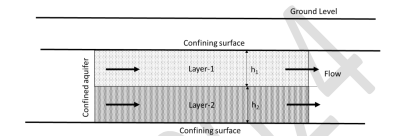
\includegraphics[width=0.6\linewidth]{figs/fig3.png}
    \caption{Third figure}
    \label{fig:third}
\end{figure}
\newpage
\begin{enumerate} 
    \item $K_x = \dfrac{K_1 h_1 + K_2 h_2}{h_1 + h_2}$
    \item $K_x = \dfrac{K_1 + K_2}{2}$
    \item $K_x = \dfrac{K_1 h_2 + K_2 h_1}{h_1 + h_2}$
    \item $K_x = \sqrt{K_1 \, K_2}$
\end{enumerate}

\item A gravity settling chamber of height 'H' and length 'L' is designed to control particulate
air pollution. In the chamber, the horizontal velocity of air flow is '$V_h$' and terminal
settling velocity of the target particle is '$V_t$'.
Which one of the following expressions is the correct concept used to calculate the
minimum size of the target particle that will be removed with $100\%$ efficiency?
 \begin{enumerate} 
  \begin{multicols}{4}
  \item $\frac{V_t}{L} = \frac{V_h}{H}$
  \item $V_h \times V_t = L \times H$
  \item $V_h = V_t \times L \times H$
  \item $\frac{V_t}{H} = \frac{V_h}{L}$
 \end{multicols}
  \end{enumerate}
  
\item Consider the function $f(x) = ln(sin(x))$.
\vspace{0.1cm}
Expand $f(x + h)$ usin Taylor's series. In this context, the correct statement(s) is/are
 \vspace{0.1cm}
\begin{enumerate}
  \item Second term in the Taylor's series i.e., the term which includes h is: h.$ln(sin(x))$
  \item First term is $ln(sin(x))$
  \item Third term in the Taylor's series i.e., the term which includes $h^2$ is: $\frac{-h^2}{2(sin(x))^2}$
  \item Third term in the Taylor's series i.e., the term which includes $h^2$ is:$\frac{2h^2}{(sin(x))^2}$
  \end{enumerate}
\item Enzymes with the class of enzymes are listed in the table.
\begin{center}
\renewcommand{\arraystretch}{1.1}
\setlength{\tabcolsep}{10pt}
\begin{tabular}{|l|l|}
\hline
\textbf{Enzyme} & \textbf{Class of Enzyme} \\ \hline
(a) Lactate dehydrogenase & (i) Isomerases \\ \hline
(b) Alanine racemase       & (ii) Transferases \\ \hline
(c) Lipase                 & (iii) Oxidoreductases \\ \hline
(d) Hexokinase             & (iv) Hydrolases \\ \hline
\end{tabular}
\end{center}
Select the correct match(es)
 \begin{enumerate} 
  \begin{multicols}{2}
  \item (a) - (iii); (b) - (i)
  \item (c) - (iv); (d) - (ii)
  \item (a) - (ii); (b) - (iv)
  \item (c) - (iii); (d) - (i)
 \end{multicols}
  \end{enumerate}
\item With reference to disinfection,which of the following statement(s) is/are $\mathbf{CORRECT}$?
\begin{enumerate}
  \item Ethanol damages lipid structures in the bacterial cell membrane.
  \item Mercuric chloride inactivates cellular enzymes containing sulfhydryl groups.
  \item Glutaraldehyde inactivates protein.
  \item Isopropyl alcohol cannot be used as a disinfectant.
  \end{enumerate}
  \vspace{0.1cm}
\item Which of the following statement(s) is/are $\mathbf{CORRECT}$?
\begin{enumerate}
  \item DNA is composed of nucleotides
  \item Five types of nitrogenous bases occur in DNA
  \item Each phosphate is attached to two deoxyribose units in a single strand of DNA.
  \item The ratio of adenine to guanine is always $1:1$ in a double stranded DNA.
  \end{enumerate}
  \newpage
\item The Streeter Phelp's oxygen sag equation for a river is based on a few assumptions.
The correct assumption(s) is/are
\begin{enumerate}
  \item At any instant the deoxygenation rate is directly proportional to the amount of
oxidizable organic material present. 
  \item At any instant the deoxygenation rate is inversely proportional to the amount of
oxidizable organic material present. 
  \item The reoxygenation rate is directly proportional to the dissolved oxygen deficit
  \item The reoxygenation rate and deoxygenation rate are directly proportional to the
saturation concentration of dissolved oxygen
  \end{enumerate}
\item Water is flowing $\mathbf{FULL}$ through a rectangular tunnel of size $3$ m (width) \(\times\) $2$ m (height).
The average velocity of flow is $1$ m/s. The frictional head loss is observed to be $1$ m per
km. Consider acceleration due to gravity (g) as $10$ m/$s^2$. The correct statement(s) is/are
\begin{enumerate}
  \item Hydraulic radius is $0.6$ m
  \item Darcy-Weisbach friction factor is $0.048$
  \item Hydraulic radius is $2$ m
  \item Darcy-Weisbach friction factor is $0.024$
  \end{enumerate}

\item Based on the ISO $14040$ methodology for Life Cycle Assessment, match the terms with
the descriptions in the table. 

\begin{center}
\renewcommand{\arraystretch}{1.3}
\setlength{\tabcolsep}{6pt} 
\begin{tabular}{|p{3cm}|p{8cm}|}
\hline
\textbf{Term} & \textbf{Description} \\ \hline
(a) Goal and Scope      & (i) Based on the product or system, the comparative unit must be carefully defined and be same for all scenarios \\ \hline
(b) Functional Unit     & (ii) The problem is described, and the objective of the study are defined \\ \hline
(c) Life Cycle \newline Inventory & (iii) Evaluates the environmental implications due to the inventorized emissions \\ \hline
(d) Impact \newline Assessment   & (iv) Process based approach and input--output approach \\ \hline
\end{tabular}
\end{center}
\begin{enumerate}  
    \begin{multicols}{4}
\item (a)-(ii); b-(i);
\item (a)-(iii), b-(i)
\item (c)-(iii), (d)-(iv)
\item (c)-(iv), (d)-(iii)
    \end{multicols}
\end{enumerate}
\item Consider the equation for a curve, $y = f(x) = x^2 + x$.

\vspace{0.1cm}
The area enclosed by the curve, the x -axis (y= $0$ line); the vertical lines passing through x = 1 and x = 2 is \underline{\hspace{1.5cm}}(rounded off to $2$ decimal places)

\vspace{0.1cm}

\item The pH of a solution containing $0.1$M of acetic acid and $0.05$ M of sodium acetate is
\underline{\hspace{1.5cm}} (rounded off to $2$ decimal places).

\vspace{0.1cm}
The pKa value of ionization of acetic acid is $4.76$.

\vspace{0.1cm}
\item The ionic strength of a solution containing 0.01M of $CaCl_2$ and $0.001$M of $Na_2SO_4$ is \underline{\hspace{1.5cm}}M (rounded off to $3$ decimal places).
\newpage
\item The concentration of Ozone corresponding to a mixing ratio of $120$ ppbv at pressure of $1$
atmosphere and temperature of 25$^\degree$C is \underline{\hspace{1.5cm}} $\mu$g/$m^3$
(rounded off to $1$ decimal place).
Atomic weight of oxygen = $16$; R= $8.314$ J/K-g.mole.

\vspace{0.1cm}
\item One million liters per day (MLD) of wastewater with a soluble BOD of $200$ mg/L is
treated in an activated sludge process. The BOD of treated wastewater is $20$ mg/L. The
observed yield coefficient of the biological system is $0.35$.

\vspace{0.1cm}
The daily biomass generation in the system is \underline{\hspace{1.5cm}} kg (an integer value).

\vspace{0.1cm}
\item An industry discharges $2$ million liters per day (MLD) of wastewater with a temperature
of $45^\degree$C and a pH of $2$, whereas the neighboring industry produces $3$ MLD of wastewater
with a temperature of $30^\degree$C and pH of $8$. If both the wastewaters are mixed and carried
through a pipeline, then the resultant pH of mixed wastewater is \underline{\hspace{1.5cm}}(rounded off
to $2$ decimal places).

Neglect buffering capacity of the system and the temperature effect on pH.

\item Consider a watershed and isohyets as shown in the figure. The average rainfall in the
watershed is \underline{\hspace{1.5cm}} mm (an integer value).
\begin{figure}[H]
    \centering
    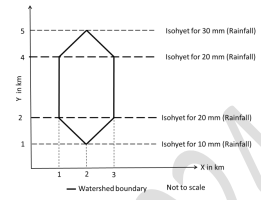
\includegraphics[width=0.4\linewidth]{figs/fig4.png}
    \caption{Fourth figure}
    \label{fig:fourth}
\end{figure}

\item With reference to the gate shown in the figure, the gate will start opening automatically
when the water level 'h' above the hinge is \underline{\hspace{1.5cm}}m
(rounded off to $2$ decimal places).
\begin{figure}[H]
    \centering
    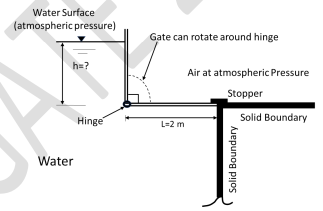
\includegraphics[width=0.4\linewidth]{figs/fig5.png}
    \caption{Fifth figure}
    \label{fig:fifth}
\end{figure}
\newpage
\item In a cyclone separator of radius $25$ cm, a particle is travelling with a gas stream at velocity
of $18$ m/s. The ratio of centrifugal force to the gravitational force acting on the particle is
\underline{\hspace{1.5cm}} (rounded off to $2$ decimal places).

Consider acceleration due to gravity (g) as $9.8$ m/$s^2$.

\vspace{0.2cm}
\item Two sources of noise, adjacent to each other in a room, have sound pressure levels of $30$
and $40$ decibel (dB). The combined sound pressure level in the room is \underline{\hspace{1.5cm}} dB
(rounded off to $2$ decimal places).

\vspace{0.1cm}
Use reference sound pressure as $20\mu$Pa.

\vspace{0.3cm}
\item An industrial stack emits $100$ g/s of CO at an effective height of 'H', where the wind
speed is $5$ m/s. At $3$ km distance downwind, the values of dispersion coefficient in y-direction and z-direction are $50$ m and $25$ m, respectively. The CO concentration at the
centerline of the plume at $3$ km distance downwind is \underline{\hspace{1.5cm}}mg/$m^3$
(rounded off to $2$
decimal places)?

\vspace{0.1cm}
Use Gaussian plume model and value of $\pi$ = $3.14$. Neglect reactions and the ground effect
of plume in the calculations.

\vspace{0.3cm}
\item Two hypothetical organic waste streams A and B are mixed prior to the composting
process. Waste-A has $2.16\%$ of C and $1.20\%$ of N. Waste-B has $19.10\%$ of C and $0.14\%$
of N. The quantity of Waste-B that should be mixed with per kg of Waste-A to achieve
the desired C:N ratio of $25$ is \underline{\hspace{1.5cm}}kg (rounded off to $2$ decimal places).

Assume both the waste streams are completely dry.

\vspace{0.3cm}
\item Food waste, paper waste and plastic waste have typical densities of $280$ kg/$m^3$
, $80$ kg/$m^3$
,
and $50$ kg/$m^3$
, respectively. The mixed waste is composed of $70\%$ food waste, $20\%$ paper
waste and $10\%$ plastic waste. The density of the mixed waste is \underline{\hspace{1.5cm}}kg/$m^3$
(rounded
off to $2$ decimal places).
Neglect compaction effect.

\vspace{0.3cm}
\item For a biodegradable waste with a chemical formula $C_{50}H_{100}N_{40}$, the maximum
theoretical methane production per ton of waste is \underline{\hspace{1.5cm}} kg (rounded off to $2$ decimal
places).
Assume $100\%$ anaerobic conversion. Atomic weights of C-$12$; H-$1$; O-$16$; N-$14$

\vspace{0.3cm}
\item A person consumes $2.5$ liters of water per day. The water quality test indicated that the
supplied water has a Pb concentration of $0.6$ mg/L. If the weight of the person is $75$ kg,
the exposure level for Pb for this person from this drinking water source is \underline{\hspace{1.5cm}} mg/kg/day (rounded off to $2$ decimal places).

\vspace{0.3cm}
\item In a region, total annual consumption of gasoline is $30.6$ million tons. The land required
for growing sugarcane to produce enough bioethanol to replace the gasoline completely
is \underline{\hspace{1.5cm}} $km^2$ (an integer value).

Ethanol energy equivalent is $67\%$ of gasoline, gasoline density is $850$ kg/$m^3$
, yield of
bioethanol produced from sugarcane per hectare of land is $3750$ L, and 1 $km^2$ = $100$ hectares.

 \vspace{0.3cm}
\item Initially a bottle contained $400$ g of ethanol. Half of ethanol was used by a student for
preparing the stock solution in an environmental chemistry laboratory just before summer
vacation of $90$ days. After completing the procedure, the student left the bottle uncorked.
If the unsealed bottle losses ethanol at a rate of $0.5$ g/day, the ethanol that will be left in
the bottle at the end of the summer vacation is \underline{\hspace{1.5cm}} g (an integer value).

 \end{enumerate}
\end{document}